%  Proceeding paper para Engineering Proceedings (MDPI) -- ECP 2026
%  Plantilla oficial MDPI (ACS), https://www.mdpi.com/authors/latex
%  Compilar: latexmk -pdf main.tex   (o pdflatex + bibtex + pdflatex x2)

%=================================================================
\documentclass[engproc,proceedingpaper,submit,moreauthors]{Definitions/mdpi}

%=================================================================
% MDPI internal commands - do not modify
\firstpage{1}
\makeatletter
\setcounter{page}{\@firstpage}
\makeatother
\pubvolume{1}
\issuenum{1}
\articlenumber{0}
\pubyear{2026}
\copyrightyear{2026}
\datereceived{ }
\daterevised{ }
\dateaccepted{ }
\datepublished{ }

%=================================================================
% Paquetes y comandos propios
\usepackage{algorithm}
\usepackage{algpseudocode}
\algrenewcommand\algorithmicrequire{\textbf{Input:}}
\algrenewcommand\algorithmicensure{\textbf{Output:}}
\usetikzlibrary{positioning}

\DeclareMathOperator*{\argmin}{arg\,min}
\newcommand{\sd}[1]{\,(#1)}        % desviación estándar entre paréntesis

%=================================================================
\Title{Triple Resolutive Approach: A Repository of Five Combinatorial Optimization Problems with Exact and Metaheuristic Solutions $^{\dagger}$}

\Author{Benjamín Peña Díaz * and Gustavo Gatica}

\AuthorNames{Benjamín Peña Díaz and Gustavo Gatica}

\address[1]{%
Faculty of Engineering, Universidad Andres Bello, Santiago, Chile; ggatica@unab.cl}

\corres{Correspondence: benja.diaz.2911@gmail.com}

\firstnote{Presented at the 5th International Electronic Conference on Processes (ECP 2026), Online, 20--22 October 2026; Available online: \url{https://sciforum.net/event/ECP2026}.}

\abstract{Comparative studies of metaheuristics usually report which algorithm wins, but seldom which component explains the result. This work presents a repository that implements three progressive Tabu Search (TS) configurations for five classical combinatorial optimization problems: the 0/1 knapsack, the traveling salesman problem (TSP), the capacitated vehicle routing problem (CVRP), permutation flowshop scheduling and job shop scheduling. The configurations are basic (fixed tabu list), intermediate (dynamic tabu list and soft restart) and advanced (frequency memory, adaptive penalization and informed diversification). A total of 360 runs (24 instances, three configurations, five seeds) show that the advanced configuration reduces the average gap to the best-known solution from 6.50\% to 3.40\%, with the largest gains in CVRP (19.22\% to 6.38\%) and TSP (2.42\% to 1.22\%), at 3.9 times the computing time. The repository includes instance loaders, exact reference models, an experiment orchestrator and report generators to support replication.}

\keyword{tabu search; metaheuristics; combinatorial optimization; knapsack problem; traveling salesman problem; vehicle routing; flowshop scheduling; job shop scheduling; reproducible research}

%%%%%%%%%%%%%%%%%%%%%%%%%%%%%%%%%%%%%%%%%%
\begin{document}

%%%%%%%%%%%%%%%%%%%%%%%%%%%%%%%%%%%%%%%%%%
\section{Introduction}

Combinatorial optimization problems arise in logistics, manufacturing, finance and resource planning. Most of them are NP-hard \cite{garey1979computers}, which has driven the development of exact algorithms and, above all, of metaheuristics that deliver good solutions in practical computing times \cite{gendreau2010handbook,blum2003metaheuristics}. Tabu Search (TS) \cite{glover1986future,glover1989tabu,glover1990tabu} records recent moves in a tabu list to avoid revisiting solutions and to escape from local optima, and it can be enriched with long-term memory, aspiration criteria, restarts and adaptive penalties \cite{glover1997tabu}.

Most studies either compare TS against other families of metaheuristics or propose highly specialized variants for a single problem \cite{gendreau1994tabu,cordeau2001unified,nowicki1996fast}. As Hooker warns \cite{hooker1995testing}, this competitive testing tells which algorithm wins, but not which component explains the result. A methodological gap remains: code bases that illustrate the internal progression of TS, from a basic configuration to an advanced one, over several heterogeneous problems, with reproducible experiments and unified metrics.

This paper addresses that gap. The name \emph{Triple Resolutive Approach} refers to the three progressive TS configurations that are applied to each problem. The contributions are as follows:
\begin{enumerate}
\item Fifteen TS modules in Python (five problems, three configurations) behind a single interface;
\item An experiment orchestrator that runs the 360 experiments, stores every result as JSON and generates the consolidated tables;
\item A quantitative analysis of the effect of each configuration on five classical problems;
\item A repository, including exact reference models, that can be extended to new problems or algorithms without changing the existing infrastructure.
\end{enumerate}

%%%%%%%%%%%%%%%%%%%%%%%%%%%%%%%%%%%%%%%%%%
\section{Materials and Methods}

\subsection{Problems and Benchmark Instances}

Table~\ref{tab:problems} summarizes the five problems in their standard form, together with the solution encoding, the neighbourhood of the basic configuration and the constructive heuristic that provides the initial solution. The same initial solution is used by the three configurations of a problem.

\begin{table}[H]
\caption{Problems, solution encodings, basic neighbourhoods, constructive heuristics and instance sets.\label{tab:problems}}
\begin{adjustwidth}{-\extralength}{0cm}
\small
\begin{tabularx}{\fulllength}{@{}m{2.6cm}m{2.5cm}m{2.9cm}m{2.3cm}Lm{3.4cm}@{}}
\toprule
\textbf{Problem} & \textbf{Objective} & \textbf{Solution Encoding} & \textbf{Neighbourhood} & \textbf{Initial Solution} & \textbf{Instances}\\
\midrule
0/1 knapsack \cite{martello1990knapsack} & max.\ total profit & binary vector & bit flip & greedy by profit/weight ratio & 5; 100 items; generated \cite{pisinger2005hard}\\
TSP \cite{applegate2006traveling} & min.\ tour length & tour (permutation) & 2-opt \cite{croes1958method} & nearest neighbour & 5; 51--100 cities; TSPLIB \cite{reinelt1991tsplib}\\
CVRP \cite{toth2002vehicle} & min.\ total distance & set of routes & relocate & Clarke--Wright savings \cite{clarke1964scheduling} & 4; 50--150 customers \cite{christofides1979vehicle}\\
Permutation flowshop \cite{pinedo2016scheduling} & min.\ makespan & job permutation & adjacent swap & NEH \cite{nawaz1983heuristic} & 5; 20$\times$5 to 50$\times$10; Taillard \cite{taillard1993benchmarks}\\
Job shop \cite{garey1976complexity} & min.\ makespan & priority sequence of operations & adjacent swap & Giffler--Thompson decoder \cite{giffler1960algorithms} & 5; 10$\times$5 to 15$\times$10 \cite{fisher1963probabilistic,lawrence1984resource}\\
\bottomrule
\end{tabularx}
\end{adjustwidth}
\end{table}

The TSP, CVRP, flowshop and job shop instances are published benchmarks, and their best-known solutions (BKS) are the values reported in the literature. The flowshop instances are the first instance of five of Taillard's classes \cite{taillard1993benchmarks} (\texttt{ta001}, \texttt{ta011}, \texttt{ta021}, \texttt{ta031} and \texttt{ta041}), regenerated from their published seeds, and their BKS are optimal makespans. The knapsack instances were generated following Pisinger's class of uncorrelated instances with similar weights \cite{pisinger2005hard} (100 items, weights in $[45, 55]$, profits in $[1, 100]$ and capacity 2500); their reference values are optimal and were verified by dynamic programming.

\subsection{Three Levels of Tabu Search}

The three configurations expose the same interface, \texttt{solve(instance\_data, ...)}, and each one inherits the components of the previous level:
\begin{itemize}
\item \textbf{TS-Basic} uses a tabu list of fixed length, the neighbourhood of Table~\ref{tab:problems}, the selection of the best non-tabu move and the standard aspiration criterion, by which a tabu move is accepted when it improves the incumbent. It has no stochastic component.
\item \textbf{TS-Intermediate} uses a dynamic tabu list whose length is redrawn in $[T_{\min}, T_{\max}]$ every $\Delta$ iterations, an idea taken from robust TS \cite{taillard1991robust} and related to reactive TS \cite{battiti1994reactive}. In the two scheduling problems it adds a soft restart, which applies three random swaps to the incumbent after $L$ non-improving iterations. In CVRP it adds intra-route 2-opt moves.
\item \textbf{TS-Advanced} adds a frequency memory $\phi$ that counts how often each component (item, edge, customer, job position or job pair) takes part in the accepted moves. Moves are ranked by the objective value modified by a penalty $\lambda \, \Phi$, where $\Phi$ is the frequency of the components involved. The weight $\lambda \in [0, \lambda_{\max}]$ increases after $L$ non-improving iterations, to diversify, and decreases when the incumbent improves, to intensify. When the search stagnates for $L$ iterations, a diversification step is triggered: a double-bridge move \cite{martin1992large} in TSP, and a perturbation of the incumbent or a stronger penalty in the other problems. In CVRP this level also adds inter-route swaps.
\end{itemize}

Algorithm~\ref{alg:ts} summarizes the advanced level and marks the steps that each level introduces, and Table~\ref{tab:params} lists the parameters. The design follows the framework of Glover and Laguna \cite{glover1997tabu}. The parameters were set by hand and were not tuned per instance.

\begin{algorithm}[H]
\caption{Tabu Search, advanced level. Steps marked [I] are introduced at the intermediate level and steps marked [A] at the advanced level.}\label{alg:ts}
\small
\begin{algorithmic}[1]
\Require instance; tabu range $[T_{\min}, T_{\max}]$; period $\Delta$; stagnation limit $L$; penalty bound $\lambda_{\max}$; iteration budget $I_{\max}$; seed $s$
\Ensure best solution found $x^{*}$ and its value $f(x^{*})$
\State $x \leftarrow$ constructive heuristic; \ $x^{*} \leftarrow x$; \ $\mathcal{T} \leftarrow \emptyset$; \ $\phi \leftarrow 0$; \ $\lambda \leftarrow \lambda_{0}$; \ $e \leftarrow 0$
\For{$it = 1, \ldots, I_{\max}$}
\If{$it \bmod \Delta = 0$} $|\mathcal{T}| \leftarrow$ random integer in $[T_{\min}, T_{\max}]$ \Comment{[I] dynamic list}
\EndIf
\State $x' \leftarrow \argmin_{x'' \in \mathcal{N}(x)} f(x'') + \lambda \, \Phi(x'')$ \ s.t.\ $\mathrm{move}(x'') \notin \mathcal{T}$ \textbf{or} $f(x'') < f(x^{*})$ \Comment{[A] penalty}
\State $\phi(\mathrm{move}(x')) \leftarrow \phi(\mathrm{move}(x')) + 1$; \ $\mathcal{T} \leftarrow \mathcal{T} \cup \{\mathrm{move}(x')\}$; \ $x \leftarrow x'$ \Comment{[A] frequency memory}
\If{$f(x) < f(x^{*})$} $x^{*} \leftarrow x$; \ $e \leftarrow 0$; \ decrease $\lambda$ \Comment{[A] intensify}
\Else \ $e \leftarrow e + 1$
\EndIf
\If{$e \geq L$} increase $\lambda$; \ $x \leftarrow \mathrm{perturb}(x^{*}, \phi)$; \ $e \leftarrow 0$ \Comment{[I] restart, [A] informed}
\EndIf
\EndFor
\State \Return $x^{*}$
\end{algorithmic}
\end{algorithm}

\begin{table}[H]
\caption{Parameters of the three levels: tabu list length $|\mathcal{T}|$ or range $[T_{\min}, T_{\max}]$, period $\Delta$, iteration budget $I_{\max}$, stagnation limit $L$ and penalty bound $\lambda_{\max}$. A dash indicates that the level has no restart for that problem.\label{tab:params}}
\small
\begin{tabularx}{\textwidth}{@{}l cc cccc ccccc@{}}
\toprule
 & \multicolumn{2}{c}{\textbf{TS-Basic}} & \multicolumn{4}{c}{\textbf{TS-Intermediate}} & \multicolumn{5}{c}{\textbf{TS-Advanced}}\\
\cmidrule(lr){2-3}\cmidrule(lr){4-7}\cmidrule(l){8-12}
\textbf{Problem} & $|\mathcal{T}|$ & $I_{\max}$ & Range & $\Delta$ & $I_{\max}$ & $L$ & Range & $\Delta$ & $I_{\max}$ & $L$ & $\lambda_{\max}$\\
\midrule
Knapsack & 10 & 500  & [5, 15] & 50  & 1000 & --  & [5, 15] & 50  & 2000 & 200 & 2.0\\
TSP      & 10 & 1000 & [5, 20] & 100 & 2000 & --  & [7, 25] & 150 & 3000 & 300 & 5.0\\
CVRP     & 10 & 1500 & [7, 20] & 150 & 3000 & --  & [7, 25] & 200 & 5000 & 400 & 3.0\\
Flowshop & 10 & 2000 & [5, 20] & 200 & 4000 & 500 & [5, 20] & 200 & 5000 & 500 & 3.0\\
Job shop & 10 & 2500 & [5, 15] & 100 & 1000 & 200 & [5, 15] & 100 & 1500 & 250 & 3.0\\
\bottomrule
\end{tabularx}
\end{table}

\subsection{Repository Architecture}

Figure~\ref{fig:architecture} shows the data flow of the repository. The folder \texttt{instances/} stores the 24 instances, and \texttt{tabu\_search/} holds the fifteen modules, one per problem and level. In \texttt{src/}, the orchestrator \texttt{main.py} runs any subset of the experiments, \texttt{loader.py} parses the instances and their reference values, \texttt{runner.py} loads each module by dynamic import and executes it, \texttt{metrics.py} computes the gap, and \texttt{reporter.py} aggregates the results into CSV and \LaTeX{} tables. Every module returns the same dictionary, with the keys \texttt{value}, \texttt{solution}, \texttt{iterations}, \texttt{time\_s} and \texttt{history}. For this reason the orchestrator treats the five problems uniformly, and a new problem or algorithm only requires a new module. Each run writes its own folder in \texttt{output/}, with \texttt{resultado.json} (metrics and convergence history) and \texttt{solucion.txt} (best solution found). The folder \texttt{models/} contains reference formulations of the five problems in AMPL and exact solvers in Python: dynamic programming for the knapsack and the Held--Karp algorithm \cite{held1962dynamic} for the TSP.

\begin{figure}[H]
\centering
\begin{tikzpicture}[
    node distance=0.55cm and 1.2cm,
    comp/.style={draw, rounded corners=2pt, align=center, font=\footnotesize\ttfamily,
                 text width=3.4cm, minimum height=1.25cm, fill=gray!8},
    etapa/.style={font=\scriptsize\itshape, text=gray!90!black},
    fl/.style={->, >=stealth, thick}]
  \node[comp] (inst) {instances/\\{\scriptsize .kp .tsp .vrp .fsp .jss}};
  \node[comp, right=of inst] (src) {src/\\{\scriptsize main.py, loader.py, runner.py}};
  \node[comp, right=of src] (ts) {tabu\_search/\\{\scriptsize 15 solve() modules}};
  \node[comp, below=of ts] (out) {output/\\{\scriptsize resultado.json, solucion.txt}};
  \node[comp, left=of out] (rep) {src/\\{\scriptsize metrics.py, reporter.py}};
  \node[comp, left=of rep] (res) {results/, notebooks/\\{\scriptsize tables and figures}};
  \draw[fl] (inst) -- node[above, etapa]{load} (src);
  \draw[fl] (src) -- node[above, etapa]{run} (ts);
  \draw[fl] (ts) -- node[right, etapa]{store} (out);
  \draw[fl] (out) -- node[above, etapa]{aggregate} (rep);
  \draw[fl] (rep) -- node[above, etapa]{generate} (res);
\end{tikzpicture}
\caption{Architecture of the repository and data flow. The orchestrator loads the instances, runs the fifteen TS modules and stores the results, from which the metrics, tables and figures are generated.\label{fig:architecture}}
\end{figure}

\subsection{Experimental Design}

Each of the 24 instances was solved by the three configurations with five independent seeds (42, 123, 456, 789 and 1337), which gives 360 runs. The stopping criterion is the iteration budget of Table~\ref{tab:params}. Performance is measured by the gap with respect to the reference value,
\begin{equation}
\mathrm{GAP}\,(\%) = 100 \times
\begin{cases}
(f^{*} - \mathrm{BKS})/\mathrm{BKS}, & \text{for minimization},\\
(\mathrm{BKS} - f^{*})/\mathrm{BKS}, & \text{for maximization},
\end{cases}
\label{eq:gap}
\end{equation}
where $f^{*}$ is the best value found by the algorithm. The mean and the sample standard deviation over the five seeds are reported. The experiments were run in Python on a laptop with an 11th-generation Intel Core i7 processor and 8 GB of RAM.

%%%%%%%%%%%%%%%%%%%%%%%%%%%%%%%%%%%%%%%%%%
\section{Results and Discussion}

\subsection{Overall Effect of the Levels}

Table~\ref{tab:results} reports the results for every instance. Averaged over the five problems, the gap decreases from 6.50\% with TS-Basic to 4.00\% with TS-Intermediate and to 3.40\% with TS-Advanced, a relative reduction of 48\%. TS-Advanced obtains a lower mean gap than TS-Basic in 17 of the 24 instances, the same gap in six and a higher gap in one. The mean computing time grows from 4.93 s to 19.10 s, a factor of 3.9.

The reduction is not uniform. Most of it (2.50 of 3.10 percentage points) takes place between the basic and the intermediate level, and it comes almost entirely from CVRP. The advanced level contributes the remaining 0.60 points and lowers the mean gap of every problem except flowshop, by between 0.02 points in the knapsack and 1.34 points in CVRP. Since TS-Basic has no stochastic component, its five runs coincide and its standard deviation is zero.

\subsection{Analysis by Problem}

\textbf{Knapsack.} The three levels stay below 0.7\% in every instance and reach the optimum in three of the five. The greedy initial solution and the exhaustive bit-flip neighbourhood leave little room for improvement. Figure~\ref{fig:convergence}a shows that TS-Basic stalls at 0.66\% after four iterations, whereas the other two levels reach 0.08\% at iteration 73.

\textbf{TSP.} TS-Basic obtains gaps between 0.94\% and 3.91\%. The dynamic list of TS-Intermediate improves the result only in the two \texttt{eil} instances. The largest gain appears with TS-Advanced, whose double-bridge restart lowers the gap of \texttt{kroA100} from 2.99\% to 0.76\%. This move changes four edges at once and lets the search leave basins of attraction in which the 2-opt moves remain trapped, which produces the stepwise descent of Figure~\ref{fig:convergence}b.

\textbf{CVRP.} This is the problem where the progression has the greatest effect. With relocate moves only, TS-Basic stays at 26.26\% in \texttt{vrpnc1}. TS-Intermediate, which adds intra-route 2-opt, reduces the mean gap from 19.22\% to 7.72\%. TS-Advanced reaches 6.38\%, at 7.5 times the computing time of TS-Intermediate. In \texttt{vrpnc4}, with 150 customers, TS-Advanced (9.16\%) does not improve on TS-Intermediate (8.70\%), which suggests that the penalty weight requires tuning in the larger instances.

\begin{table}[H]
\caption{Gap (\%) with respect to the reference value, as mean and standard deviation (in parentheses) over five seeds, and mean computing time (s). B, I and A denote TS-Basic, TS-Intermediate and TS-Advanced. The global row is the mean of the five problem means.\label{tab:results}}
\begin{adjustwidth}{-\extralength}{0cm}
\footnotesize
\begin{tabularx}{\fulllength}{@{}llcr CCC rrr@{}}
\toprule
 & & & & \multicolumn{3}{c}{\textbf{Gap (\%)}} & \multicolumn{3}{c}{\textbf{Time (s)}}\\
\cmidrule(lr){5-7}\cmidrule(l){8-10}
\textbf{Problem} & \textbf{Instance} & \textbf{Size} & \textbf{Ref.} & \textbf{B} & \textbf{I} & \textbf{A} & \textbf{B} & \textbf{I} & \textbf{A}\\
\midrule
Knapsack & knapPI\_11 & 100 & 3950 & 0.66\sd{0.00} & 0.21\sd{0.25} & 0.15\sd{0.07} & 0.01 & 0.02 & 0.06\\
 & knapPI\_12 & 100 & 3752 & 0.43\sd{0.00} & 0.43\sd{0.00} & 0.37\sd{0.13} & 0.01 & 0.02 & 0.08\\
 & knapPI\_13 & 100 & 3468 & 0.00\sd{0.00} & 0.00\sd{0.00} & 0.00\sd{0.00} & 0.01 & 0.03 & 0.08\\
 & knapPI\_14 & 100 & 3856 & 0.00\sd{0.00} & 0.00\sd{0.00} & 0.00\sd{0.00} & 0.01 & 0.02 & 0.06\\
 & knapPI\_15 & 100 & 3732 & 0.00\sd{0.00} & 0.00\sd{0.00} & 0.00\sd{0.00} & 0.01 & 0.02 & 0.08\\
 & \textit{Mean} & & & \textit{0.22} & \textit{0.13} & \textit{0.10} & \textit{0.01} & \textit{0.02} & \textit{0.07}\\
\midrule
TSP & eil51 & 51 & 426 & 1.64\sd{0.00} & 1.46\sd{0.26} & 0.56\sd{0.13} & 0.70 & 1.56 & 3.56\\
 & berlin52 & 52 & 7542 & 3.91\sd{0.00} & 3.91\sd{0.00} & 2.70\sd{0.23} & 0.86 & 1.75 & 3.54\\
 & eil76 & 76 & 538 & 2.60\sd{0.00} & 1.45\sd{0.65} & 1.15\sd{0.50} & 1.76 & 3.51 & 7.72\\
 & kroA100 & 100 & 21,282 & 2.99\sd{0.00} & 2.99\sd{0.00} & 0.76\sd{0.03} & 3.16 & 6.89 & 13.46\\
 & kroB100 & 100 & 22,141 & 0.94\sd{0.00} & 0.94\sd{0.00} & 0.94\sd{0.00} & 3.08 & 6.76 & 13.67\\
 & \textit{Mean} & & & \textit{2.42} & \textit{2.15} & \textit{1.22} & \textit{1.91} & \textit{4.09} & \textit{8.39}\\
\midrule
CVRP & vrpnc1 & 50 & 524 & 26.26\sd{0.00} & 7.94\sd{0.00} & 6.69\sd{1.14} & 0.44 & 1.49 & 12.88\\
 & vrpnc2 & 75 & 835 & 16.74\sd{0.00} & 8.67\sd{0.00} & 5.03\sd{0.75} & 1.03 & 2.56 & 27.40\\
 & vrpnc3 & 100 & 826 & 14.95\sd{0.00} & 5.59\sd{0.00} & 4.64\sd{0.75} & 3.36 & 12.46 & 75.24\\
 & vrpnc4 & 150 & 1028 & 18.94\sd{0.00} & 8.70\sd{0.00} & 9.16\sd{0.14} & 6.88 & 20.32 & 161.47\\
 & \textit{Mean} & & & \textit{19.22} & \textit{7.72} & \textit{6.38} & \textit{2.93} & \textit{9.21} & \textit{69.25}\\
\midrule
Flowshop & ta001 & 20$\times$5 & 1278 & 0.63\sd{0.00} & 0.52\sd{0.24} & 0.52\sd{0.24} & 0.84 & 1.72 & 1.88\\
 & ta011 & 20$\times$10 & 1582 & 1.71\sd{0.00} & 1.64\sd{0.67} & 1.47\sd{0.43} & 1.30 & 2.85 & 3.75\\
 & ta021 & 20$\times$20 & 2297 & 1.39\sd{0.00} & 1.63\sd{0.51} & 1.85\sd{0.28} & 2.74 & 5.68 & 6.30\\
 & ta031 & 50$\times$5 & 2724 & 0.18\sd{0.00} & 0.18\sd{0.00} & 0.18\sd{0.00} & 4.78 & 9.68 & 11.91\\
 & ta041 & 50$\times$10 & 2991 & 4.78\sd{0.00} & 4.75\sd{0.09} & 4.74\sd{0.09} & 9.01 & 17.55 & 21.80\\
 & \textit{Mean} & & & \textit{1.74} & \textit{1.74} & \textit{1.75} & \textit{3.73} & \textit{7.50} & \textit{9.13}\\
\midrule
Job shop & ft10 & 10$\times$10 & 930 & 19.78\sd{0.00} & 20.43\sd{0.74} & 19.59\sd{0.91} & 8.49 & 3.11 & 4.53\\
 & la01 & 10$\times$5 & 666 & 1.80\sd{0.00} & 2.25\sd{1.24} & 1.65\sd{0.57} & 4.12 & 1.46 & 2.23\\
 & la06 & 15$\times$5 & 926 & 6.05\sd{0.00} & 0.00\sd{0.00} & 0.00\sd{0.00} & 13.28 & 4.73 & 6.91\\
 & la11 & 20$\times$5 & 1222 & 0.00\sd{0.00} & 1.33\sd{1.57} & 0.00\sd{0.00} & 28.39 & 10.13 & 15.39\\
 & la21 & 15$\times$10 & 1046 & 16.83\sd{0.00} & 17.19\sd{0.87} & 16.35\sd{1.33} & 25.98 & 10.12 & 14.34\\
 & \textit{Mean} & & & \textit{8.89} & \textit{8.24} & \textit{7.52} & \textit{16.05} & \textit{5.91} & \textit{8.68}\\
\midrule
\textbf{Global} & & & & \textbf{6.50} & \textbf{4.00} & \textbf{3.40} & \textbf{4.93} & \textbf{5.35} & \textbf{19.10}\\
\bottomrule
\end{tabularx}
\end{adjustwidth}
\end{table}

\textbf{Flowshop.} The three levels are tied, with mean gaps of 1.74\%, 1.74\% and 1.75\%. The gap of TS-Basic ranges from 0.18\% in \texttt{ta031} to 4.78\% in \texttt{ta041}, where it improves the NEH solution by a single time unit. In \texttt{ta031} the three levels reach the same makespan in every run, and in \texttt{ta021} TS-Advanced is worse than TS-Basic. These results indicate that the adjacent-swap neighbourhood, and not the memory mechanism, limits the search; an insertion neighbourhood is the natural extension.

\textbf{Job shop.} This is the hardest problem of the set. In \texttt{ft10} and \texttt{la21} the three levels remain between 16\% and 21\% (Figure~\ref{fig:convergence}d), far from the results of specialized TS methods based on critical-path neighbourhoods \cite{nowicki1996fast}. In contrast, TS-Advanced reaches the BKS in \texttt{la06} and \texttt{la11}. TS-Intermediate is worse than TS-Basic in four of the five instances and shows a high variance. However, its iteration budget is less than half that of TS-Basic (Table~\ref{tab:params}), so this comparison is not conclusive. For the same reason, TS-Basic is the slowest level in this problem (16.05 s against 5.91 s and 8.68 s).

\begin{figure}[H]
\begin{adjustwidth}{-\extralength}{0cm}
\centering
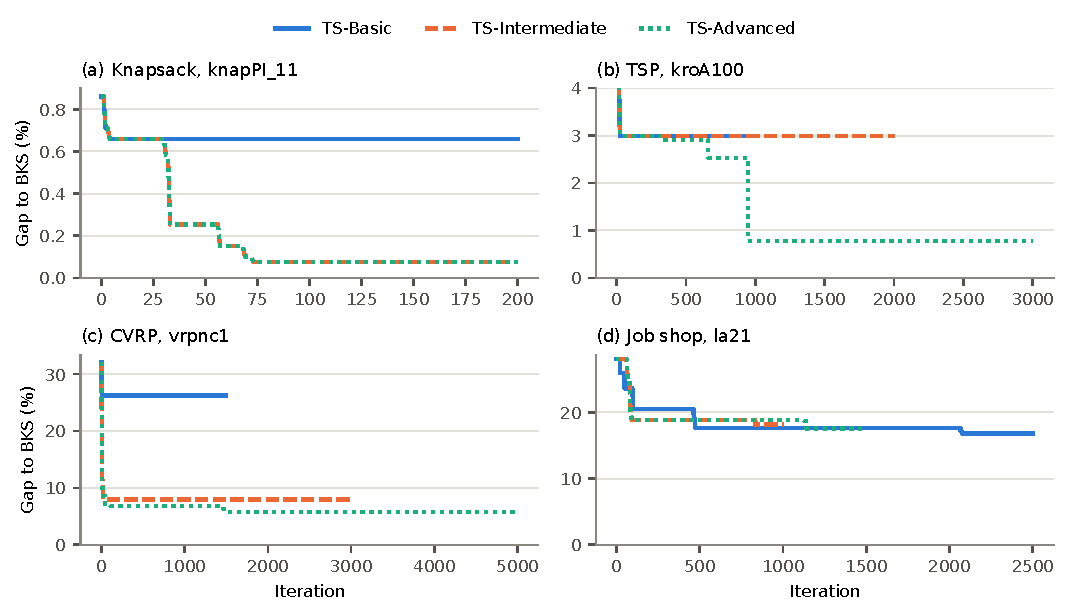
\includegraphics[width=\fulllength]{figures/convergence.pdf}
\end{adjustwidth}
\caption{Convergence of the gap of the incumbent solution for seed 42: (\textbf{a}) knapsack, instance \texttt{knapPI\_11}, first 200 iterations; (\textbf{b}) TSP, instance \texttt{kroA100}, with the vertical axis truncated at 4\% (the initial solution has a gap of 30.66\%); (\textbf{c}) CVRP, instance \texttt{vrpnc1}; (\textbf{d}) job shop, instance \texttt{la21}. Each curve ends at the iteration budget of its level.\label{fig:convergence}}
\end{figure}

\subsection{Limitations}

The three levels differ in their memory mechanisms, but also in their iteration budgets and, for the routing problems, in their neighbourhoods. The results therefore measure each configuration as a whole and do not isolate the contribution of a single mechanism; that attribution requires an ablation study with equal computing time. In addition, the parameters were not tuned, and five seeds give only a rough estimate of the variability.

%%%%%%%%%%%%%%%%%%%%%%%%%%%%%%%%%%%%%%%%%%
\section{Conclusions}

This paper presented a repository with fifteen TS implementations, three levels for each of five classical combinatorial optimization problems, and an automated experimental pipeline. Over 360 runs, the progression from the basic to the advanced level reduces the average gap by 48\%, from 6.50\% to 3.40\%, at 3.9 times the computing time. Three findings stand out. First, the benefit depends strongly on the problem: it is large in CVRP (a relative reduction of 67\%) and in TSP, marginal in the knapsack, where the constructive heuristic is already close to the optimum, and null in flowshop. Second, the neighbourhood matters at least as much as the memory: the largest improvements coincide with the levels that add intra-route 2-opt in CVRP and the double-bridge restart in TSP, whereas the three levels are tied in flowshop, where they share the adjacent-swap neighbourhood. Third, in job shop none of the levels compensates for a weak neighbourhood, and richer moves on the disjunctive graph are needed \cite{nowicki1996fast,balas1998guided}.

Future work includes an ablation study with fixed computing time, exact models for the smallest instances to obtain lower bounds, larger instances, and the extension of the repository to other problems such as graph colouring and the multidimensional knapsack.

%%%%%%%%%%%%%%%%%%%%%%%%%%%%%%%%%%%%%%%%%%
\vspace{6pt}

\authorcontributions{Conceptualization, B.P.D.; methodology, B.P.D.; software, B.P.D.; validation, B.P.D.; formal analysis, B.P.D.; investigation, B.P.D.; data curation, B.P.D.; writing---original draft preparation, B.P.D.; writing---review and editing, G.G.; visualization, B.P.D.; supervision, G.G. All authors have read and agreed to the published version of the manuscript.}

\funding{This research received no external funding.}

\institutionalreview{Not applicable.}

\informedconsent{Not applicable.}

\dataavailability{The source code, the instances, the raw results of the 360 runs and the scripts that generate the tables and figures are kept in a private repository and are available from the corresponding author on reasonable request.}

\acknowledgments{During the preparation of this manuscript, the authors used Claude (Anthropic) for programming support (experiment orchestration and generation of reports and figures) and for the translation of the text into English and its adaptation to the journal template. The authors have reviewed and edited the output and take full responsibility for the content of this publication.}

\conflictsofinterest{The authors declare no conflicts of interest.}

%%%%%%%%%%%%%%%%%%%%%%%%%%%%%%%%%%%%%%%%%%
\begin{adjustwidth}{-\extralength}{0cm}

\reftitle{References}
\bibliography{references}

\PublishersNote{}
\end{adjustwidth}
\end{document}
